\section{Problemas}

% \begin{figure}[H]
%   \centering
%   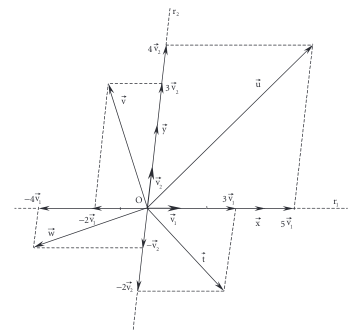
\includegraphics[width=0.6\textwidth]{./fig/fig1.38.png}
%   \caption{Vetores expressos em $\vec{v_1}$ e $\vec{v_2}$}\label{fig:fig1.38}
% \end{figure}

\question{
  Dados os vetores $\vec{u} = 2\vec{i} - 3\vec{j}$, $\vec{v} = \vec{i} -
  \vec{j}$ e $\vec{w} = -2\vec{i} + \vec{j}$, determinar:
}
\begin{itemize}
  \item \subquestion{$2\vec{u} - \vec{v}$}
    \answer{
      \begin{align*}
        2\vec{u} &= 2(2\vec{i} - 3\vec{j}) = 4\vec{i} - 6\vec{j} \\
        2\vec{u} - \vec{v} &= (4\vec{i} - 6\vec{j}) - (\vec{i} - \vec{j}) \\
        &= 4\vec{i} - 6\vec{j} - \vec{i} + \vec{j} \\
        &= (4 - 1)\vec{i} + (-6 + 1)\vec{j} \\
        &= 3\vec{i} - 5\vec{j} \\
      \end{align*}
    }

  \item \subquestion{$\vec{v} - \vec{u} + 2\vec{w}$}
    \answer{
      \begin{align*}
        \vec{v} &= \vec{i} - \vec{j} \\
        -\vec{u} &= - (2\vec{i} - 3\vec{j}) = -2\vec{i} + 3\vec{j} \\
        2\vec{w} &= 2(-2\vec{i} + \vec{j}) = -4\vec{i} + 2\vec{j} \\
        \vec{v} - \vec{u} + 2\vec{w} &= (\vec{i} - \vec{j}) + (-2\vec{i} +
        3\vec{j}) + (-4\vec{i} + 2\vec{j}) \\
        &= (\vec{i} - 2\vec{i} - 4\vec{i}) + (-\vec{j} + 3\vec{j} + 2\vec{j}) \\
        &= -5\vec{i} + 4\vec{j} \\
      \end{align*}
    }

  \item \subquestion{$\frac{1}{2}\vec{u} - 2\vec{v} - \vec{w}$}
    \answer{
      \begin{align*}
        \frac{1}{2}\vec{u} &= \frac{1}{2}(2\vec{i} - 3\vec{j}) = \vec{i} -
        \frac{3}{2}\vec{j} \\
        -2\vec{v} &= -2(\vec{i} - \vec{j}) = -2\vec{i} + 2\vec{j} \\
        -\vec{w} &= -(-2\vec{i} + \vec{j}) = 2\vec{i} - \vec{j} \\
        \frac{1}{2}\vec{u} - 2\vec{v} - \vec{w} &= (\vec{i} -
        \frac{3}{2}\vec{j}) + (-2\vec{i} + 2\vec{j}) + (2\vec{i} - \vec{j}) \\
        &= (\vec{i} - 2\vec{i} + 2\vec{i}) + \left(-\frac{3}{2}\vec{j} +
        2\vec{j} - \vec{j}\right) \\
        &= \vec{i} + \left(-\frac{3}{2} + 2 - 1\right)\vec{j} \\
        &= \vec{i} - \frac{1}{2}\vec{j} \\
      \end{align*}
    }

  \item \subquestion{$3\vec{u} - \frac{1}{2}\vec{v} - \frac{1}{2}\vec{w}$}
    \answer{
      \begin{align*}
        3\vec{u} &= 3(2\vec{i} - 3\vec{j}) = 6\vec{i} - 9\vec{j} \\
        \frac{1}{2}\vec{v} &= \frac{1}{2}(\vec{i} - \vec{j}) =
        \frac{1}{2}\vec{i} - \frac{1}{2}\vec{j} \\
        \frac{1}{2}\vec{w} &= \frac{1}{2}(-2\vec{i} + \vec{j}) = -\vec{i} +
        \frac{1}{2}\vec{j} \\
        3\vec{u} - \frac{1}{2}\vec{v} - \frac{1}{2}\vec{w} &= (6\vec{i} -
        9\vec{j}) - \left(\frac{1}{2}\vec{i} - \frac{1}{2}\vec{j}\right) -
        \left(-\vec{i} + \frac{1}{2}\vec{j}\right) \\
        &= \left(6 - \frac{1}{2} + 1\right)\vec{i} + \left(-9 + \frac{1}{2} -
        \frac{1}{2}\right)\vec{j} \\
        &= \frac{13}{2}\vec{i} - 9\vec{j} \\
      \end{align*}
    }
\end{itemize}

\newpage
\question{
  Dados os vetores $\vec{u} = (3, -1)$ e $\vec{v} = (-1, 2)$, determinar o vetor
  $\vec{x}$ tal que:
}
\begin{center}
  % First column
  \begin{minipage}[t]{0.48\textwidth}
    \begin{itemize}
      \item \subquestion{$4(\vec{u} - \vec{v}) + \frac{1}{3}\vec{x} = 2\vec{u} -
        \vec{x}$}
        \answer{
          \begin{align*}
            4(\vec{u} - \vec{v}) - 2\vec{u} &= -\vec{x} - \frac{1}{3}\vec{x} \\
            2\vec{u} - 4\vec{v} &= -\frac{4}{3}\vec{x} \\
            2(3, -1) - 4(-1, 2) &= -\frac{4}{3}\vec{x} \\
            (6, -2) - (-4, 8) &= -\frac{4}{3}\vec{x} \\
            (10, -10) &= -\frac{4}{3}\vec{x} \\
            (10, -10) &= (-\frac{4}{3}x_1, -\frac{4}{3}y_1) \\
            \vec{x} &= (-\frac{15}{2}, \frac{15}{2}) \\
          \end{align*}
        }
    \end{itemize}
  \end{minipage}
  \hfill
  % Second column
  \begin{minipage}[t]{0.48\textwidth}
    \begin{itemize}
      \item \subquestion{$3\vec{x} - (2\vec{v} - \vec{u}) = 2(4\vec{x} -
        3\vec{u})$}
        \answer{
          \begin{align*}
            3\vec{x} + (-2\vec{v} + \vec{u}) &= 8\vec{x} - 6\vec{u} \\
            3\vec{x} - 8\vec{x} &= -6\vec{u} + (2\vec{v} - \vec{u}) \\
            -5\vec{x} &= -6(3, -1) + (2(-1, 2) - (3, -1)) \\
            -5\vec{x} &= (-18, 6) + ((-2, 4) - (3, -1)) \\
            -5\vec{x} &= (-18, 6) + (-5, 5) \\
            -5\vec{x} &= (-23, 11) \\
            \vec{x} &= (\frac{23}{5}, -\frac{11}{5}) \\
          \end{align*}
        }
    \end{itemize}
  \end{minipage}
\end{center}

\question{
  Dados os pontos $A(-1, 3)$, $B(2, 5)$, $C(3, -1)$ e $O(0, 0)$, calcular:
}
\begin{center}
  \begin{itemize}
    \item \subquestion{$\overrightarrow{OA} - \overrightarrow{AB}$}
      \answer{
        \begin{align*}
          \overrightarrow{OA} &= (-1 - 0, 3 - 0) \\
          \overrightarrow{OA} &= (-1, 3) \\
          \overrightarrow{AB} &= (2 + 1, 5 - 3) \\
          \overrightarrow{AB} &= (3, 2) \\
          \overrightarrow{OA} - \overrightarrow{AB} &= (-1, 3) - (3, 2) \\
          \overrightarrow{OA} - \overrightarrow{AB} &= (-4, 1) \\
        \end{align*}
      }
    \item \subquestion{$\overrightarrow{OC} - \overrightarrow{BC}$}
      \answer{
        \begin{align*}
          \overrightarrow{OC} &= (3, -1) \\
          \overrightarrow{BC} &= (3 - 2, -1 - 5) \\
          \overrightarrow{BC} &= (1, -6) \\
          \overrightarrow{OC} - \overrightarrow{BC} &= (3, -1) - (1, -6) \\
          \overrightarrow{OC} - \overrightarrow{BC} &= (2, 5) \\
        \end{align*}
      }
    \item \subquestion{$\frac{3}{4}\overrightarrow{BA} - \overrightarrow{CB}$}
      \answer{
        \begin{align*}
          \frac{3}{4}\overrightarrow{BA} &= (\frac{3}{4}(-1 - 2), \frac{3}{4}(3 - 5)) \\
          \frac{3}{4}\overrightarrow{BA} &= (\frac{3}{4}(-3), \frac{3}{4}(-2)) \\
          \frac{3}{4}\overrightarrow{BA} &= (-\frac{9}{4}, -\frac{6}{4}) \\
          \overrightarrow{CB} &= (2 - 3, 5 + 1) \\
          \overrightarrow{CB} &= (-1, 6) \\
          \frac{3}{4}\overrightarrow{BA} - \overrightarrow{CB} &= (-\frac{9}{4}, -\frac{6}{4}) - (-1, 6) \\
          \frac{3}{4}\overrightarrow{BA} - \overrightarrow{CB} &= (-\frac{5}{4}, -\frac{15}{2}) \\
        \end{align*}
      }
  \end{itemize}
\end{center}

\question{
  Dados os vetores $\vec{u} = (2, -4)$, $\vec{v} = (-5, 1)$ e $\vec{w} = (-12,
  6)$, determinar $a_1$ e $a_2$ tais que $\vec{w} = a_1\vec{u} + a_2\vec{v}$.
}
\answer{
  \begin{aligned*}
    (-12, 6) &= a_1(2, -4) + a_2(-5, 1) \\
    &= (2a_1, -4a_1) + (-5a_2, a_2) \\
    &= (2a_1 - 5a_2, -4a_1 + a_2) \\[1em]
    & \begin{cases}
      2a_1 - 5a_2 = -12 \\
      -4a_1 + a_2 = 6
    \end{cases} \\[1em]
    \text{Solution:} \quad & a_1 = -1 \quad \text{e} \quad a_2 = 2
  \end{aligned*}
}

\newpage
\question{
  Dados os pontos $A(3, -4)$ e $B(-1, 1)$ e o vetor $\vec{v} = (-2, 3)$,
  calcular:
}
\begin{center}
  % First column
  \begin{minipage}[t]{0.48\textwidth}
    \begin{itemize}
      \item \subquestion{$(B - A) + 2\vec{v}$}
        \answer{
          \begin{aligned*}
            ((-1, 1) - (3, -4)) + 2(-2, 3) \\
            (-4, 5) + (-4, 6) \\
            (-8, 11) \\
          \end{aligned*}
        }
      \item \subquestion{$(A - B) - \vec{v}$}
        \answer{
          \begin{aligned*}
            ((3, -4) - (-1, 1)) - (-2, 3) \\
            (4, -5) - (-2, 3) \\
            (6, -8) \\
          \end{aligned*}
        }
    \end{itemize}
  \end{minipage}
  \hfill
  % Second column
  \begin{minipage}[t]{0.48\textwidth}
    \begin{itemize}
      \item \subquestion{$B + 2(B - A)$}
        \answer{
          \begin{aligned*}
            (-1, 1) + 2((-1, 1) - (3, -4)) \\
            (-1, 1) + 2(-4, 5) \\
            (-1, 1) + (-8, 10) \\
            (-9, 11) \\
          \end{aligned*}
        }
      \item \subquestion{$3\vec{v} - 2(A - B)$}
        \answer{
          \begin{aligned*}
            3(-2, 3) - 2((3, -4) - (-1, 1)) \\
            (-6, 9) - 2(4, -5) \\
            (-6, 9) - (8, -10) \\
            (-14, 19) \\
          \end{aligned*}
        }
    \end{itemize}
  \end{minipage}
\end{center}

\question{
  Sejam os pontos $A(-5, 1)$ e $B(1, 3)$. Determinar o vetor $\vec{v}$ tal que:
}
\begin{center}
  % First column
  \begin{minipage}[t]{0.48\textwidth}
    \begin{itemize}
      \item \subquestion{$B = A + 2\vec{v}$}
        \answer{
          \begin{aligned*}
            2\overrightarrow{v} &= B - A \\
            2\overrightarrow{v} &= (1 + 5, 3 - 1) \\
            2\overrightarrow{v} &= (6, 2) \\
            \overrightarrow{v} &= (3, 1) \\
          \end{aligned*}
        }
        \begin{figure}[H]
          \centering
          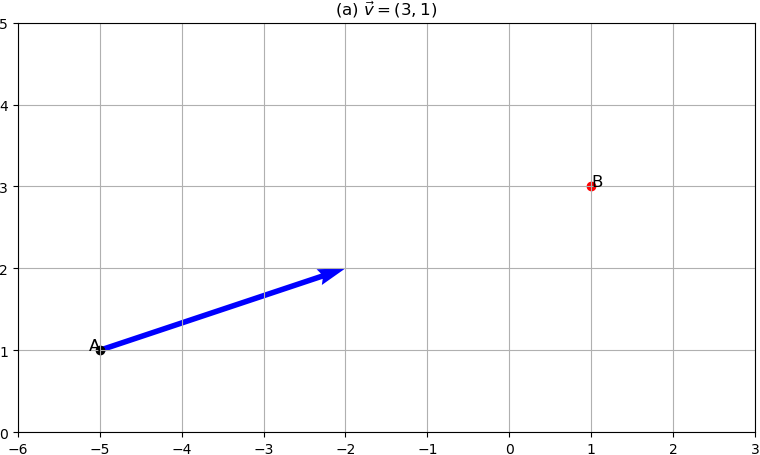
\includegraphics[width=1\textwidth]{./fig/q6a.png}
        \end{figure}
    \end{itemize}
  \end{minipage}
  \hfill
  % Second column
  \begin{minipage}[t]{0.48\textwidth}
    \begin{itemize}
      \item \subquestion{$A = B + 3\vec{v}$}
        \answer{
          \begin{aligned*}
            3\overrightarrow{v} &= A - B \\
            3\overrightarrow{v} &= (-5 - 1, 1 - 3) \\
            3\overrightarrow{v} &= (-6, -2) \\
            \overrightarrow{v} &= \left(-2, -\frac{2}{3}\right) \\
          \end{aligned*}
        }
        \begin{figure}[H]
          \centering
          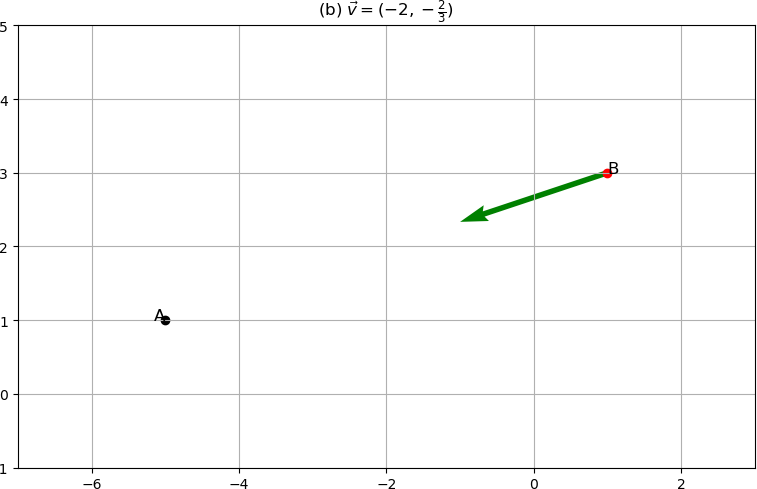
\includegraphics[width=1\textwidth]{./fig/q6b.png}
        \end{figure}
    \end{itemize}
  \end{minipage}
\end{center}

\newpage
\question{
  Qual ponto inicial do segmento orientado que representa o vetor $\vec{v} =
  (-1, 3)$, sabendo que sua extremidade está em $(3, 1)$? Representar
  graficamente esse segmento.
}
\answer{
  \begin{aligned*}
    \overrightarrow{v} &= B - A \\
    (v_x, v_y) &= (3 - A_x, 1 - A_y) \\
    v_x &= 3 - A_x \\
    v_x - 3 &= - A_x \\
    3 + 1 &= A_x \\
    4 &= A_x \\
    v_y &= 1 - A_y \\
    v_y - 1 &= - A_y \\
    1 - 3 &= A_y \\
    -2 &= A_y \\
    A &= (4, -2) \\
  \end{aligned*}
  \begin{figure}[H]
    \centering
    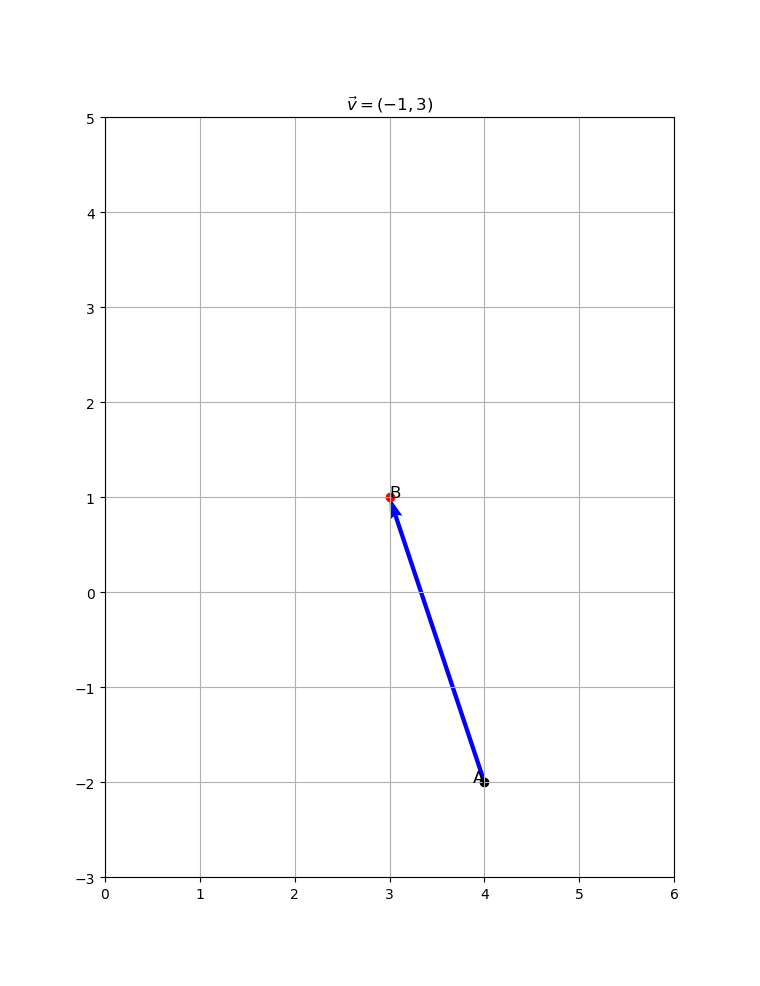
\includegraphics[width=0.5\textwidth]{./fig/q7.png}
  \end{figure}
}

\newpage
\question{
  Sejam os pontos $P(2, 3)$, $Q(4, 2)$ e $R(3, 5)$.
}
\begin{center}
  % First column
  \begin{minipage}[t]{0.47\textwidth}
    \begin{itemize}
      \item \subquestion{Representar em um mesmo gráfico os vetores posição de $\vec{u}$, $\vec{v}$ e $\vec{w}$ de modo que $Q = P + \vec{u}$, $R = Q + \vec{v}$ e $P = R + \vec{w}$}
        \answer{
          \begin{figure}[H]
            \centering
            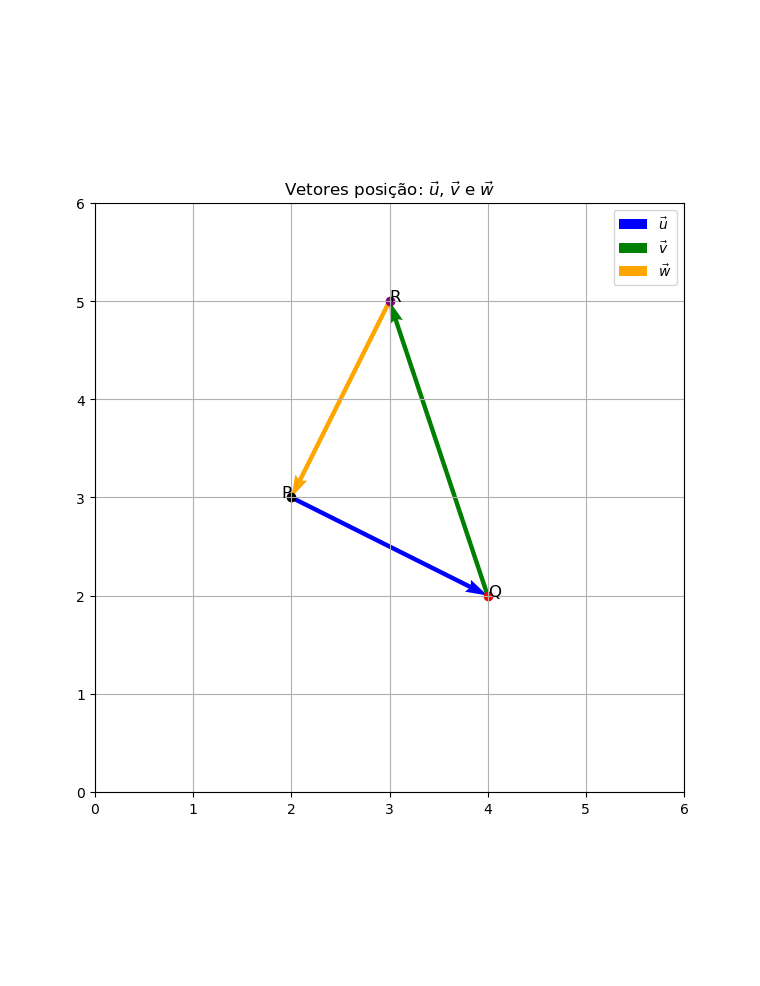
\includegraphics[width=1\textwidth]{./fig/q8.png}
          \end{figure}
        }
    \end{itemize}
  \end{minipage}
  \hfill
  % Second column
  \begin{minipage}[t]{0.52\textwidth}
    \begin{itemize}
      \item \subquestion{Determinar $\vec{u} + \vec{v} + \vec{w}$}
        \answer{
          \begin{aligned*}
            \overrightarrow{u} &= Q - P = (4-2, 2-3) = (2, -1) \\
            \overrightarrow{v} &= R - Q = (3-4, 5-2) = (-1, 3) \\
            \overrightarrow{w} &= P - R = (2-3, 3-5) = (-1, -2) \\
            \overrightarrow{u} + \overrightarrow{v} + \overrightarrow{w} &= (2-1-1, -1+3-2) \\
            &= (0, 0)
          \end{aligned*}
        }
    \end{itemize}
  \end{minipage}
\end{center}

\newpage
\question{
  Encontrar o vértice oposto a $B$, no paralelogramo $ABCD$, para:
}
\begin{center}
  % First column
  \begin{minipage}[t]{0.48\textwidth}
    \begin{itemize}
      \item \subquestion{$A(−3, −1)$, $B(4, 2)$ e $C(5, 5)$}
        \answer{
          \begin{aligned*}
            \overrightarrow{BA} &= A - B = (-3 - 4,\ -1 - 2) \\
                                &= (-7,\ -3) \\
            D &= C + \overrightarrow{BA} \\
              &= (5,\ 5) + (-7,\ -3) \\
              &= (-2,\ 2) \\
          \end{aligned*}
        }
    \end{itemize}
  \end{minipage}
  \hfill
  % Second column
  \begin{minipage}[t]{0.48\textwidth}
    \begin{itemize}
      \item \subquestion{$A(5, 1)$, $B(7, 3)$ e $C(3, 4)$}
        \answer{
          \begin{aligned*}
            \overrightarrow{BA} &= A - B = (5 - 7,\ 1 - 3) \\
                                &= (-2,\ -2) \\
            D &= C + \overrightarrow{BA} \\
              &= (3,\ 4) + (-2,\ -2) \\
              &= (1,\ 2) \\
          \end{aligned*}
        }
    \end{itemize}
  \end{minipage}
\end{center}

\question{
  Sabendo que $A(1, -1)$, $B(5, 1)$ e $C(6, 4)$ são vértices de um
  paralelogramo, determinar o quarto vértice de cada um dos três paralelogramos
  possíveis de serem formados.
}
\begin{center}
  % First column
  \begin{minipage}[t]{0.75\textwidth}
    \begin{itemize}
      \item \subquestion{1º Caso: $AB$ e $AC$ como lados consecutivos}
        \answer{
          \begin{aligned}
            \text{Seja } D_1(x,y) \\
            \vec{AB} &= (5 - 1, 1 - (-1)) = (4, 2) \\
            \vec{AC} &= (6 - 1, 4 - (-1)) = (5, 5) \\
            \vec{AD_1} &= \vec{AB} + \vec{AC} = (9, 7) \\
            D_1 &= A + \vec{AD_1} = (1, -1) + (9, 7) = (10, 6)
          \end{aligned}
        }
      \item \subquestion{2º Caso: $BA$ e $BC$ como lados consecutivos}
        \answer{
          \begin{aligned}
            \vec{BA} &= (1 - 5, -1 - 1) = (-4, -2) \\
            \vec{BC} &= (6 - 5, 4 - 1) = (1, 3) \\
            \vec{BD_2} &= \vec{BA} + \vec{BC} = (-3, 1) \\
            D_2 &= B + \vec{BD_2} = (5, 1) + (-3, 1) = (2, 2)
          \end{aligned}
        }
      \item \subquestion{3º Caso: $AB$ e $BC$ como lados consecutivos}
        \answer{
          \begin{aligned}
            \vec{AB} &= (4, 2),\quad \vec{BC} = (1, 3) \\
            \text{Queremos } \vec{D_3A} &= \vec{BC} \\
            D_3 &= A - \vec{BC} = (1, -1) - (1, 3) = (0, -4)
          \end{aligned}
        }
    \end{itemize}
  \end{minipage}
\end{center}

\newpage
\question{
  Dados os pontos $A(-3, 2)$ e $B(5, -2)$, determinar os pontos $M$ e $N$
  pertencentes ao segmento $AB$ tais que $\frac{AM}{AB} = \frac{1}{2}$ e
  $\frac{AN}{AB} = \frac{2}{3}$. Construir o gráfico, marcando os pontos $A$,
  $B$, $M$, $N$ e $P$, em que $P$ seja tal que $\frac{AP}{AB} = \frac{3}{2}$.
}
\begin{center}
  % First column
  \begin{minipage}[t]{0.48\textwidth}
    \begin{itemize}
      \item \subquestion{Cálculo do vetor $\overrightarrow{AB}$ e pontos $M$, $N$, $P$}
        \answer{
          \begin{aligned}
            \overrightarrow{AB} &= B - A = (8, -4) \\
            \overrightarrow{AM} &= \frac{1}{2}\overrightarrow{AB} = \left(\frac{8}{2}, \frac{-4}{2}\right) = (4, -2) \\
            M &= A + \overrightarrow{AM} = (1, 0) \\
            \overrightarrow{AN} &= \frac{2}{3}\overrightarrow{AB} = \left(\frac{16}{3}, \frac{-8}{3}\right) \\
            N &= A + \overrightarrow{AN} = \left(\frac{7}{3}, -\frac{2}{3}\right) \\
            \overrightarrow{AP} &= \frac{3}{2}\overrightarrow{AB} = (12, -6) \\
            P &= A + \overrightarrow{AP} = (9, -4) \\
          \end{aligned}
        }
    \end{itemize}
  \end{minipage}
  \hfill
  % Second column
  \begin{minipage}[t]{0.51\textwidth}
    \begin{itemize}
      \item \subquestion{Representação gráfica}
        \answer{
          \begin{figure}[H]
            \centering
            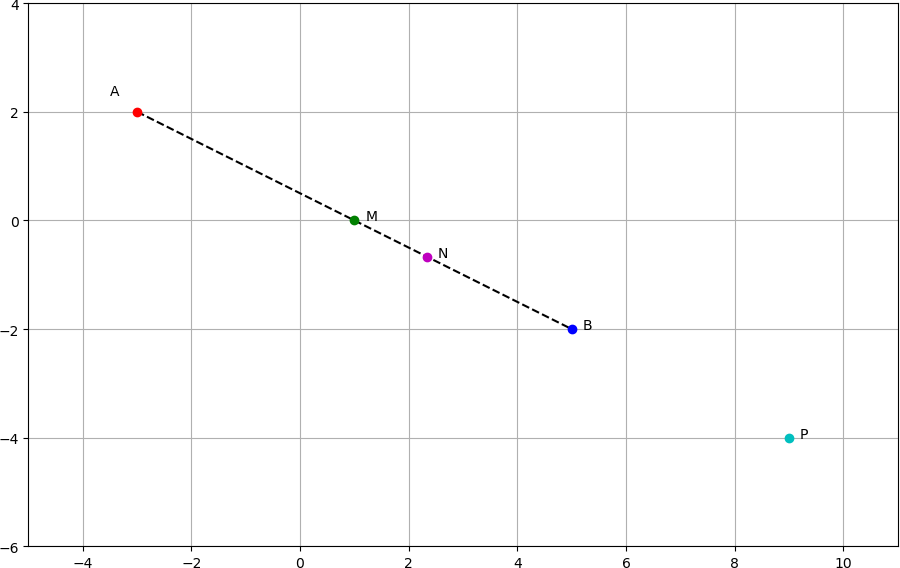
\includegraphics[width=1\textwidth]{./fig/q11.png}
          \end{figure}
        }
    \end{itemize}
  \end{minipage}
\end{center}

\question{
  Sendo $A(-2, 3)$ e $B(6, -3)$ extremidades de um segmento, determinar:
}
\begin{center}
  % Primeira coluna - Parte (a)
  \begin{minipage}[t]{0.48\textwidth}
    \begin{itemize}
      \item \subquestion{Pontos $C$, $D$ e $E$ que dividem o segmento $AB$ em
        quatro partes de mesmo comprimento}
        \answer{
          \begin{aligned}
            \overrightarrow{AB} &= B - A = (8, -6) \\
            \overrightarrow{AC} &= \frac{1}{4}\overrightarrow{AB} = (2, -1.5) \\
            C &= A + \overrightarrow{AC} = (0, \frac{3}{2}) \\
            \overrightarrow{AD} &= \frac{2}{4}\overrightarrow{AB} = (4, -3) \\
            D &= A + \overrightarrow{AD} = (2, 0) \\
            \overrightarrow{AE} &= \frac{3}{4}\overrightarrow{AB} = (6, -4.5) \\
            E &= A + \overrightarrow{AE} = (4, -\frac{3}{2}) \\
          \end{aligned}
        }
    \end{itemize}
  \end{minipage}
  \hfill
  % Segunda coluna - Parte (b)
  \begin{minipage}[t]{0.48\textwidth}
    \begin{itemize}
      \item \subquestion{Pontos $F$ e $G$ que dividem o segmento $AB$ em
        três partes de mesmo comprimento}
        \answer{
          \begin{aligned}
            \overrightarrow{AF} &= \frac{1}{3}\overrightarrow{AB} = \left(\frac{8}{3}, -2\right) \\
            F &= A + \overrightarrow{AF} = \left(\frac{2}{3}, 1\right) \\
            \overrightarrow{AG} &= \frac{2}{3}\overrightarrow{AB} = \left(\frac{16}{3}, -4\right) \\
            G &= A + \overrightarrow{AG} = \left(\frac{10}{3}, -1\right) \\
          \end{aligned}
        }
    \end{itemize}
  \end{minipage}
\end{center}

\newpage
\question{
  O ponto $P$ pertence ao segmento de extremos $A(x_1, y_1)$ e $B(x_2, y_2)$, e
  a sua distância ao ponto $A$ é a terça parte da sua distância ao ponto $B$.
  Expressar as coordenadas de $P$ em função das coordenadas de $A$ e $B$.
}
\answer{
  \begin{aligned}
    &AP = \frac{1}{3}PB \Rightarrow PB = 3AP \\
    &\frac{AP}{PB} = \frac{1}{3} \Rightarrow \frac{AP}{AB} = \frac{1}{4} \\
    &\overrightarrow{AP} = \frac{1}{4}\overrightarrow{AB} \\
    &P = A + \frac{1}{4}\overrightarrow{AB} \\
    &P_x = x_1 + \frac{1}{4}(x_2 - x_1) = \frac{3x_1 + x_2}{4} \\
    &P_y = y_1 + \frac{1}{4}(y_2 - y_1) = \frac{3y_1 + y_2}{4} \\
    &P\left(\frac{3x_1 + x_2}{4}, \frac{3y_1 + y_2}{4}\right) \\
  \end{aligned}
}

\question{
  Dados os vetores $\vec{u} = (1, -1)$, $\vec{v} = (-3, 4)$ e $\vec{w} = (8, -6)$, calcular:
}
\begin{center}
  % Primeira coluna
  \begin{minipage}[t]{0.48\textwidth}
    \begin{itemize}
      \item \subquestion{$|\vec{u}|$}
        \answer{
          $\sqrt{1^2 + (-1)^2} = \sqrt{2}$
        }
      
      \item \subquestion{$|\vec{w}|$}
        \answer{
          $\sqrt{8^2 + (-6)^2} = \sqrt{64 + 36} = 10$
        }
      
      \item \subquestion{$|2\vec{u} - \vec{w}|$}
        \answer{
          \begin{aligned}
            2\vec{u} - \vec{w} &= (2,-2) - (8,-6) = (-6,4) \\
            |2\vec{u} - \vec{w}| &= \sqrt{(-6)^2 + 4^2} = \sqrt{52} = 2\sqrt{13}
          \end{aligned}
        }
      
      \item \subquestion{$\frac{\vec{v}}{|\vec{v}|}$}
        \answer{
          \begin{aligned}
            |\vec{v}| &= \sqrt{(-3)^2 + 4^2} = 5 \\
            \frac{\vec{v}}{|\vec{v}|} &= \left(-\frac{3}{5}, \frac{4}{5}\right)
          \end{aligned}
        }
    \end{itemize}
  \end{minipage}
  \hfill
  % Segunda coluna
  \begin{minipage}[t]{0.48\textwidth}
    \begin{itemize}
      \item \subquestion{$|\vec{v}|$}
        \answer{
          $\sqrt{(-3)^2 + 4^2} = \sqrt{9 + 16} = 5$
        }
      
      \item \subquestion{$|\vec{u} + \vec{v}|$}
        \answer{
          \begin{aligned}
            \vec{u} + \vec{v} &= (1,-1) + (-3,4) = (-2,3) \\
            |\vec{u} + \vec{v}| &= \sqrt{(-2)^2 + 3^2} = \sqrt{13}
          \end{aligned}
        }
      
      \item \subquestion{$|\vec{w} - 3\vec{u}|$}
        \answer{
          \begin{aligned}
            \vec{w} - 3\vec{u} &= (8,-6) - (3,-3) = (5,-3) \\
            |\vec{w} - 3\vec{u}| &= \sqrt{5^2 + (-3)^2} = \sqrt{34}
          \end{aligned}
        }
      
      \item \subquestion{$\left|\frac{\vec{u}}{|\vec{u}|}\right|$}
        \answer{
          \begin{aligned}
            |\vec{u}| &= \sqrt{2} \\
            \left|\frac{\vec{u}}{|\vec{u}|}\right| &= \left|\frac{\vec{u}}{\sqrt{2}}\right| = \frac{|\vec{u}|}{\sqrt{2}} = \frac{\sqrt{2}}{\sqrt{2}} = 1
          \end{aligned}
        }
    \end{itemize}
  \end{minipage}
\end{center}

\newpage
\question{
  Calcular os valores de $a$ para que o vetor $\vec{u} = (a, -2)$ tenha módulo
  4.
}
\answer{
  \begin{aligned}
    |\vec{u}| &= 4 \\
    \sqrt{a^2 + (-2)^2} &= 4 \\
    \sqrt{a^2 + 4} &= 4 \\
    a^2 + 4 &= 16 \\
    a^2 &= 12 \\
    a &= \pm\sqrt{12} \\
    a &= \pm 2\sqrt{3} \\
  \end{aligned}
}

\question{
  Calcular os valores de $a$ para que o vetor $\vec{u} = \left(a,
  \frac{1}{2}\right)$ seja unitário.
}
\answer{
  \begin{aligned}
    |\vec{u}| &= 1 \\
    \sqrt{a^2 + \left(\frac{1}{2}\right)^2} &= 1 \\
    \sqrt{a^2 + \frac{1}{4}} &= 1 \\
    a^2 + \frac{1}{4} &= 1 \\
    a^2 &= \frac{3}{4} \\
    a &= \pm\sqrt{\frac{3}{4}} \\
    a &= \pm\frac{\sqrt{3}}{2} \\
  \end{aligned}
}

\newpage
\question{
  Encontrar um ponto $P$ do eixo $Ox$ de modo que sua distância ao ponto $A(2,
  -3)$ seja igual a 5.
}
\answer{
  \begin{aligned}
    \text{Como } P &\text{ pertence ao eixo } Ox, \\
    P &= (x, 0) \\
    d(P,A) &= 5 \\
    \sqrt{(x-2)^2 + (0-(-3))^2} &= 5 \\
    \sqrt{(x-2)^2 + 9} &= 5 \\
    (x-2)^2 + 9 &= 25 \\
    (x-2)^2 &= 16 \\
    x-2 &= \pm 4 \\
    x &= 2 \pm 4 \\
    \Rightarrow x &= 6 \quad \text{ou} \quad x = -2
  \end{aligned}
  
  \begin{center}
    P(6, 0) \quad \text{e} \quad P(-2, 0)
  \end{center}
  
  \begin{figure}[H]
    \centering
    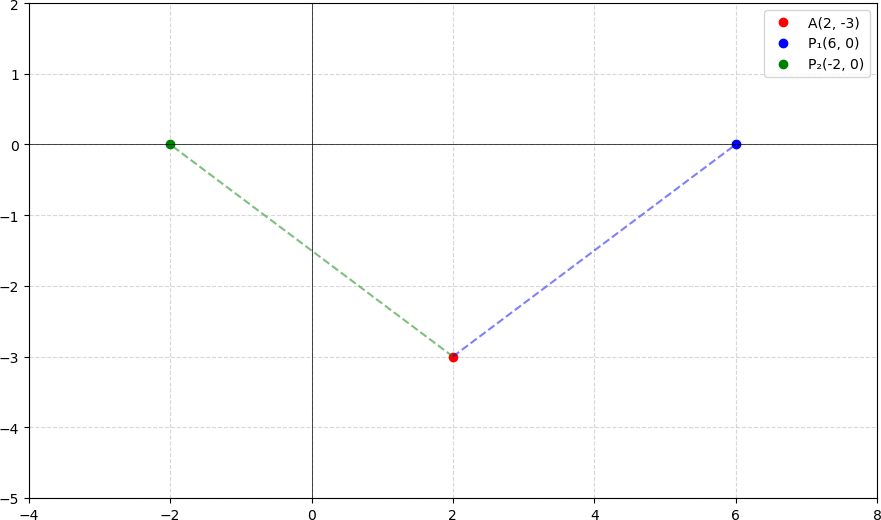
\includegraphics[width=0.8\textwidth]{./fig/q17.png}
  \end{figure}
}
